\section{Vorkenntnisabfrage}
\label{sec:Vorkenntnisabfrage}
\subsection{Skala und Struktur der Umfrage}
Um die technischen Vorkenntnisse des Entwicklungsteams zu ermitteln wird eine Umfrage durchgeführt.
Die Ergebnisse fließen als Faktor in die Entscheidungsfindung und Auswahl der Entscheidungsalternativen ein.
Durch Beachtung der Vorkenntnisse kann in der Entwicklung mehr Zeit für Umsetzung der Anforderungen aufgewendet werden, die sonst in das Erlernen neuer Technologien aufgewendet würde.

Die Skala für die Vorkenntnisabfrage umfasst vier Antwortmöglichkeiten, dessen Bedeutungen genau definiert sind und auch bei der Umfrage den Teilnehmern kommuniziert wurde.
Die Antwortmöglichkeiten können auch in eine numerische / ordinale Skala übersetzt werden, da der jeweilige Kenntnisstand auch einen Nutzen in der Entscheidungsfindung ausdrückt.
Außerdem besteht eine Rangordnung in den Antwortmöglichkeiten.

\begin{itemize}
	\item keine - noch nie mit der Programmiersprache / Technologie gearbeitet
	\item wenig - schon mal ein Tutorial durchgearbeitet bzw. eine kleine Anwendung erstellt bzw. in einer Vorlesung kennengelernt
	\item mittel - öfters mit der Programmiersprache / Technologie gearbeitet und selbstständige Problemlösung bei technischen Problemen
	\item viel - häufige Verwendung und sicherer Umgang bei Implementierung und Verwendung Bibliotheken und Frameworks
\end{itemize}

Die Umfrage ist in verschiedene Fragen bzw. Gruppen aufgeteilt, welche mehrere Technologien beinhaltet.
So kann zu der Technologie ein Kontext gegeben werden, wie z.B. eine Komponente in der Drei-Schichten-Architektur, in der die vorgestellten Technologien verwendet werden.
Pro abgefragter Technologie kann nur eine Einschätzung abgegeben werden.

\subsection{Programmiersprachen}
Die Antworten und die Verteilung der Vorkenntnisse für Programmiersprachen sind in \autoref{fig:programmiersprachen}.
Die verschieden Programmiersprachen wurden ausgewählt, da diese häufig Anwendung in der Webentwicklung finden.
Java und Python werden überwiegend für die Entwicklung von Server Anwendungen verwendet. Der größte Unterschied zwischen ihnen ist, dass Java eine stark typisierte Compiler-Sprache ist und Python eine schwach typisierte Interpretersprache ist.
JavaScript und TypeScript werden sowohl für die Entwicklung von dynamischen Browser-Anwendungen verwendet, als auch für Serveranwendungen.
TypeScript ist eine Art Super-JavaScript-Sprache, die in jeden beliebigen JavaScript Standard compiliert werden kann. 
TypeScript bietet zudem auch Typsicherheit, welche JavaScript nicht bietet.
Dennoch ist der JavaScript Syntax valides TypeScript \autocite[vgl.][]{Microsoft.od}.

\begin{figure}[H]
	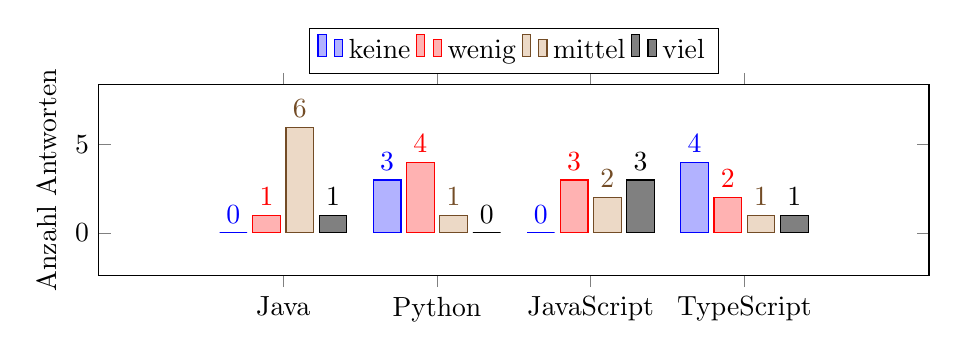
\begin{tikzpicture}
	\begin{axis}[
	ybar,
	enlargelimits=0.4,
	%legend style={at={(0.5,-0.15)},
	%	anchor=north,legend columns=-1},
	legend style={legend columns=-1,at={(0.5,1.3)},anchor=north},
	ylabel={Anzahl Antworten},
	symbolic x coords={Java,Python,JavaScript,TypeScript},
	xtick=data,
	nodes near coords,
	nodes near coords align={vertical},
	width = \linewidth,
	height = 4cm
	]
	\addplot coordinates {(Java,0) (Python,3) (JavaScript,0) (TypeScript,4)};
	\addplot coordinates {(Java,1) (Python,4) (JavaScript,3) (TypeScript,2)};
	\addplot coordinates {(Java,6) (Python,1) (JavaScript,2) (TypeScript,1)};
	\addplot coordinates {(Java,1) (Python,0) (JavaScript,3) (TypeScript,1)};
	\legend{keine,wenig,mittel,viel}
	\end{axis}
	\end{tikzpicture}
	\caption{Vorkenntnisse - Programmiersprachen}
	\label{fig:programmiersprachen}
\end{figure}

\subsection{Datenbanken}
Die Vorkenntnisse zu den Datenbanken sind in \autoref{fig:datenbank} dargestellt. Die präsentierten Datenbanken unterstützen Geo-Datenverarbeitung.
PostgreSQl ermöglicht Geo-Daten Verarbeitung mit der Erweiterung PostGIS. MariaDB, Oracle und IBM DB2 unterstützen direkt Geo-Daten Verarbeitung \autocite[vgl.][]{PostGIS.od} \autocite[vgl.][]{MariaDB.od-b} \autocite[vgl.][]{Oracle.od} \autocite{IBM.od}.
Zu unterscheiden ist, dass PostgreSQL und MariaDB kostenlose Open Source Produkte sind.
Demgegenüber sind Oracle und IBM DB2 kommerzielle Kosten behaftete Produkte.

\begin{figure}[H]
	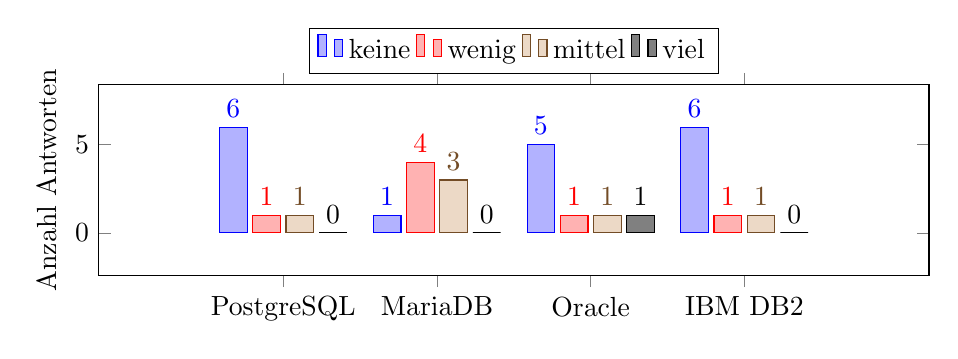
\begin{tikzpicture}
	\begin{axis}[
	ybar,
	enlargelimits=0.4,
	%legend style={at={(0.5,-0.15)},
	%	anchor=north,legend columns=-1},
	legend style={legend columns=-1,at={(0.5,1.3)},anchor=north},
	ylabel={Anzahl Antworten},
	symbolic x coords={PostgreSQL,MariaDB,Oracle,IBM DB2},
	xtick=data,
	nodes near coords,
	nodes near coords align={vertical},
	width = \linewidth,
	height = 4cm
	]
	\addplot coordinates {(PostgreSQL,6) (MariaDB,1) (Oracle,5) (IBM DB2,6)};
	\addplot coordinates {(PostgreSQL,1) (MariaDB,4) (Oracle,1) (IBM DB2,1)};
	\addplot coordinates {(PostgreSQL,1) (MariaDB,3) (Oracle,1) (IBM DB2,1)};
	\addplot coordinates {(PostgreSQL,0) (MariaDB,0) (Oracle,1) (IBM DB2,0)};
	\legend{keine,wenig,mittel,viel}
	\end{axis}
	\end{tikzpicture}
	\caption{Vorkenntnisse - Datenbanken}
	\label{fig:datenbank}
\end{figure}

\subsection{Webapplikationsframeworks - Server}
Die Vorkenntnisse zu den Server-Webapplikationsframeworks sind in \autoref{fig:backend} dargestellt. Die präsentierten Frameworks sind populär zum Erstellen der Server-Komponenten.
ExpressJS ist ein Framework für die JavaScript Laufzeitumgebung Node.js.
Spring Boot ist ein Framework für Java Anwendungen. Spring Boot integriert auch den \ac{ORM} Hibernate \autocite[vgl.][]{Pivotal.od}.
Django und Flask sind Frameworks für Python. Django hat einen integrierten \ac{ORM} und Flask ermöglicht dies durch eine Erweiterung welches auf dem \ac{ORM} SQLAlchemy basiert \autocite[vgl.][]{Pallets.od} \autocite{Django.od}.
Alle genannten \ac{ORM} unterstützen die Verarbeitung von Geo-Daten, solange die verwendete Datenbank dies unterstützt.

\begin{figure}[H]
	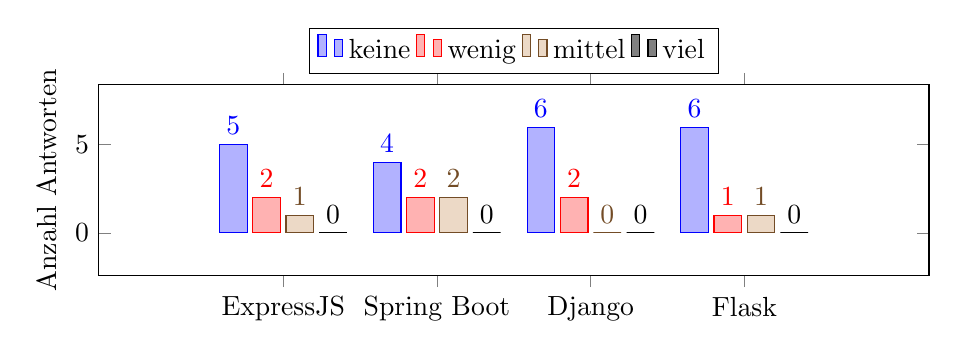
\begin{tikzpicture}
	\begin{axis}[
	ybar,
	enlargelimits=0.4,
	%legend style={at={(0.5,-0.15)},
	%	anchor=north,legend columns=-1},
	legend style={legend columns=-1,at={(0.5,1.3)},anchor=north},
	ylabel={Anzahl Antworten},
	symbolic x coords={ExpressJS,Spring Boot,Django,Flask},
	xtick=data,
	nodes near coords,
	nodes near coords align={vertical},
	width = \linewidth,
	height = 4cm
	]
	\addplot coordinates {(ExpressJS,5) (Spring Boot,4) (Django,6) (Flask,6)};
	\addplot coordinates {(ExpressJS,2) (Spring Boot,2) (Django,2) (Flask,1)};
	\addplot coordinates {(ExpressJS,1) (Spring Boot,2) (Django,0) (Flask,1)};
	\addplot coordinates {(ExpressJS,0) (Spring Boot,0) (Django,0) (Flask,0)};
	\legend{keine,wenig,mittel,viel}
	\end{axis}
	\end{tikzpicture}
	\caption{Vorkenntnisse - Server Webapplikationsframeworks}
	\label{fig:backend}
\end{figure}

\subsection{Webapplikationsframeworks - Frontend}
Die Vorkenntnisse zu den Webapplikationsframeworks sind in \autoref{fig:frontend} dargestellt. Die dargestellten Frameworks sind populär zum Erstellen der Frontend-Komponenten.
Alle vorgestellten Frameworks bis auf Angular basieren auf JavaScript.
Angular basiert auf TypeScript und benötigt einen Kompilierung zu JavaScript, welche mit einem Build-System erfolgt \autocite[vgl.][]{Google.od}.
AngularJS ist der Vorgänger zu Angular.
OpenUI5 bringt entgegen der anderen Frameworks auch direkt benutzbare Oberflächen Komponenten mit, was den Aufwand zur Integration von \ac{CSS}-Frameworks bzw. Anpassungen von \ac{CSS} erspart \autocite[vgl.][]{SAP.od}.

\begin{figure}[H]
	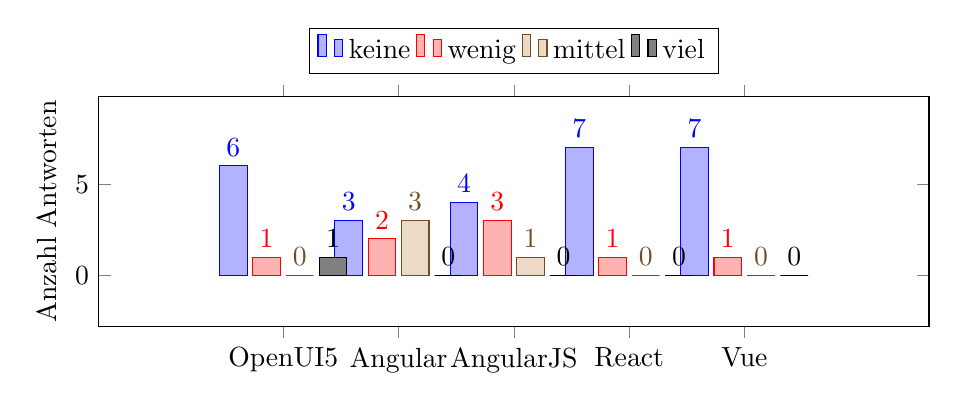
\begin{tikzpicture}
	\begin{axis}[
	ybar,
	enlargelimits=0.4,
	%legend style={at={(0.5,-0.15)},
	%	anchor=north,legend columns=-1},
	legend style={legend columns=-1,at={(0.5,1.3)},anchor=north},
	ylabel={Anzahl Antworten},
	symbolic x coords={OpenUI5,Angular,AngularJS,React,Vue},
	xtick=data,
	nodes near coords,
	nodes near coords align={vertical},
	width = \linewidth,
	height = 4.5cm
	]
	\addplot coordinates {(OpenUI5,6) (Angular,3) (AngularJS,4) (React,7) (Vue,7)};
	\addplot coordinates {(OpenUI5,1) (Angular,2) (AngularJS,3) (React,1) (Vue,1)};
	\addplot coordinates {(OpenUI5,0) (Angular,3) (AngularJS,1) (React,0) (Vue,0)};
	\addplot coordinates {(OpenUI5,1) (Angular,0) (AngularJS,0) (React,0) (Vue,0)};
	\legend{keine,wenig,mittel,viel}
	\end{axis}
	\end{tikzpicture}
	\caption{Vorkenntnisse - Webapplikationsframeworks}
	\label{fig:frontend}
\end{figure}